\chapter{Introduction}
This chapter will introduce this dissertation's subject area, present the purpose of the project and introduce the overarching aims and objectives. Some words used in this document may have several meanings therefore definitions for their meaning in this document has also been provided.


\section{Subject Area}
A significant share of today's network traffic, consists of game networking. This is due to the emence amount of data that fundamentally, has to be sent from client to client (or server) in order to keep a simulation synchronised between several participants. The general aim of any real-time simulation, such as an online multiplayer video-game, is for any action that is performed by one participant, to be replicated within the simulation of all other participants. For example in an online multiplayer game that allows for movement of a character with a press of a button, if this button is pressed by one player, all players should see this character move in their instances of the game, from their own perspectives. There are several ways in which this can be achieved.

The most common way in which a simulation is synchronised across several users, involves introducing a trusted 3rd party entity, such as a dedicated server, that would essentially determine the ``Real'' state of the simulation at any given time. Each client participating in a game instance, would submit their changes to this server which would then implement them into it's own state after checking that these changes are valid. The ``Real'' state would be broadcast periodically to each client so that everyone can update their local simulations to what is received from the server. Introducing a central entity like this provides a lot of advantages for both the players and developers. Some examples of advantages include relative fairness in latency between all players and effective implementation of a cheat prevention system that is possible because the developers control how the server works.

While this solution provides a lot of benefits to the playerbase of a game, it may not always be the best solution. In fact, the cost that is associated with the deployment of these servers can be unjustifiable for smaller projects such as indie titles. Some sources such as \mycite{zenke2008} claim that the cost of bringing an MMO to market are close to \$50 million and a large majority of this cost would be used for renting server space.

The game servers must be capable of handling a large amount of network traffic and must be powerful enough to run many simulation instances and broadcast the state of each many times a second. What makes this issue worse, is that if not enough of these servers are deployed, the experience of all players is compromised through large differences in player ping. This means that the rented server space not only has to be very powerful, but also available in as many regions of the world as possible.

An alternative for developers who do not have the budget, or find game servers to be a risky investment, is to allow player to connect to each other's game clients directly. Despite introducing some compromises, providing a service that lets players play with each other directly, may also introduce some new advantages for the players as well as the developers. There are two main methods of achieving a synchronised simulation this way; the peer to peer model and the client hosted model. The focus of this dissertation is to identify the positive and negative attributes of each networking model and to discuss the different issues that are introduced along with techniques to fix them.


\section{Project Purpose}
Most AAA games that are released to the modern game market, have gameplay features that utilise internet functionality. This type of network integration ranges from, giving the player an in-game option and showing them how many players have chosen a given choice (an example of this can be seen below in the game Life is Strange by Square Enix) to multiplayer-only reaction-based competitive gameplay (for example a screenshot from Ovewatch by Blizzard can be found below).
\begin{figure}[!h]
  \centering
\subfloat[Screenshot of choices in Life is Strange. Image from: IGN]{
    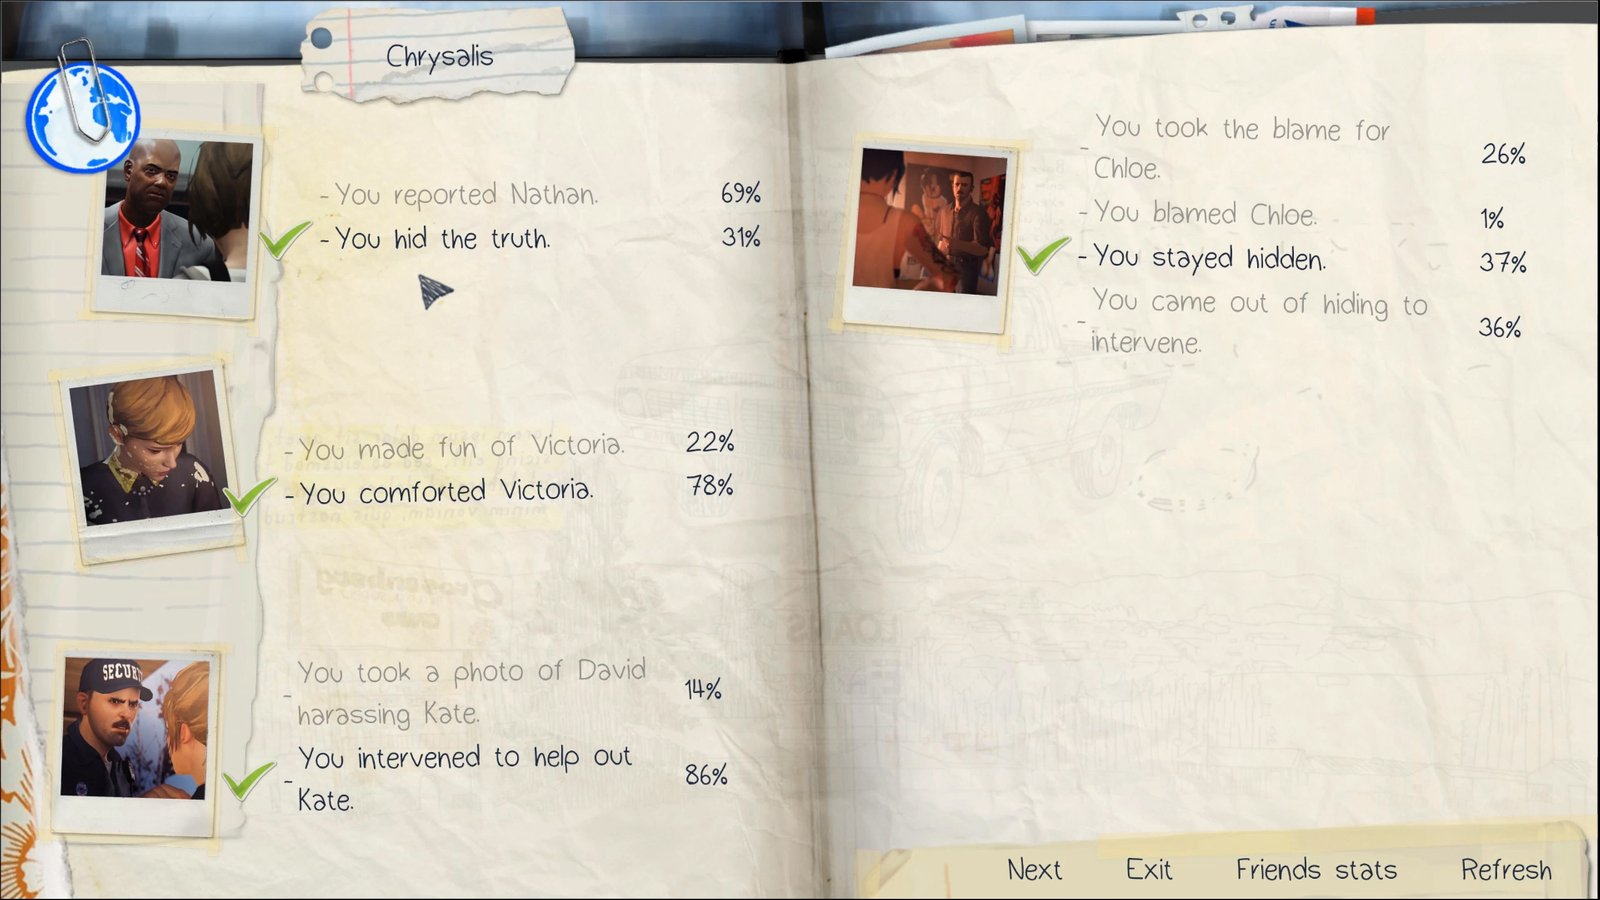
\includegraphics[width=0.45\textwidth]{Examples/Life_is_Strange}
  }
  \qquad
  \subfloat[Screenshot of Overwatch gameplay. Image from: Game Informer]{
    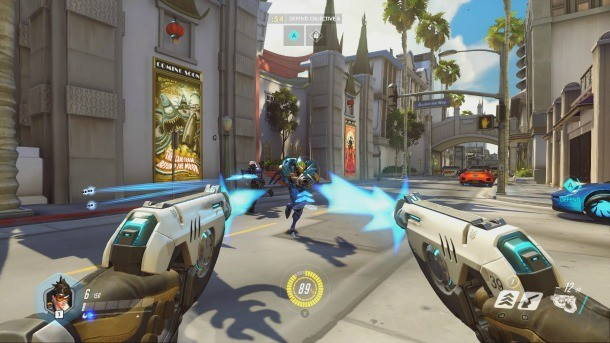
\includegraphics[width=0.45\textwidth]{Examples/Overwatch}
  }
\end{figure}

Games like the examples above are very high-budget AAA projects that are designed and developed by large teams with access to expensive technologies and worldwide servers. The access to the technology and budget that is needed for such large-scale developement projects, is simply out of reach of smaller indie developers and therefore most of the popular indie titles are simple, single-player experiances mostly focused on storytelling.

This is also likely due to how fundamentally different the programming approach must be with networking in mind, when compared to a simple single-player, one-instance game. The internet is unpredicatble, packets can arrive late or not even arrive at all, what happens when a player loses connection? There are so many new questions that have to be anwsered that for most indie developers, it doesn't seem worthwhile to spend so much time on a networking infrastructure for a game and gamble if there are even going to be enough active players so that they can play together when the game is released. This project exists to investigate just how unpredictable gaming over a network can be and just how should the networking logic be implemented to provide the best experience for the players. The developement project will also investigate just how difficult it is to implement real-time networking into a game and the final product could serve as a template for anyone attempting to create a real-time multiplayer experence without the expensive maintenance costs.


\newpage
\section{Aims and Objectives}
The aim of this dissertation is to compare examples of different methods of implementing server-less, real-time networking. It will also investigate into methods of dealing with common issues that fundamentally arrise in computer networking.
\\\\
These aims can be devided into three seperate objectives:
\begin{enumerate}
\item Investigate the common practices and techniques used in modern multiplayer games
  \\\\
  There are many different techniques that are employed to counteract the problems that naturally arrise when developing any network-enabled application. Potential issues that exist in computer network communications will be identified through the investigation of how these challenges are tackled in popular AAA games.

  The networking models that are used in the industry in these projects, will be analysed for why these choices were made by the developers.


\item Implement the peer to peer and client hosted networking models as a C++ library.
  \\\\
  The focus of this project is on server-less, real-time networking. Two commonly used strategies, that are used in the industry to support this idea, have been identified; peer to peer and client hosting. Both startegies strive for the same goal, however fundamentally employ different methods of achieving this.
  The workings of each model's networking logic, will be implemented from scratch so that any configurable variables can be easily controlled and any unnecessary bloat, unrelated to this project's investigation, does not effect the results.

\item Investigate issues spawned from computer network communication using the implemented networking models in my library.
  \\\\
  When sending packets during any computer network communication, many things have to be considered. Firstly, any transfer of information can never be instant; there is always some kind of delay. Secondly, without external systems in place, there is no guarantee that any given message packet has arrived at it's intended destination. It is possible that a valid route could not be found or the packet was intercepted. Finally, even if a packet does successfully arrive at it's intended destination, it is impossible to accurately predict the amount of time that this has taken. It is possible that messages sent at a constant rate arrive at the destination sparadically or even out of order to which they were sent in.
  Any one of these properties of computer network communications can have negative effects on both the application sending and receiving any information. These properties will be analysed for when they can occur and how they can be dealt with.
\end{enumerate}


\newpage
\section{Basic concepts and terminolory}
First of all, it is important to define some basic concepts and terminology that will be used throughout this document.
\\
\\
\textbf{Client}: Within the context of this document, a client can be defined as a piece of software responsible to running the game (i.e. game client). A client can also be defined as a computer interacting with a server, however it is possible to run two different instances of a game client on a single machine. This can also be described as a networking endpoint.
\\
\\
\textbf{Online Multiplayer Game}: A video game can be defined as a simulation of a certain scenario that can be manipulated by the player of the game. When talking about online multiplayer games, it can be thought of as a simulation that runs on several clients connected by a network (e.g. LAN or the Internet) that is to be synchronised. When one player performs an action that effects the state of the simulation, this action should also be seen by all participants of this particular simulation instance and therefore the simulation should remain in the same state across all participating clients. Due to the nature of this paper, when discussing games or simulations that use the network, it can be assumed that the given instance would be played by N > 1 participants.
\\
\\
\textbf{Ping}: In network connections, the ping between different clients refers to the shortest amount of time that is needed for one client to send information to another and receive a response from this client. One client sends a ``ICMP echo request'' to another networked client (e.g. a game server). The receiving client, then responds with an ``ICMP echo reply'' back to the original device. The time between sending the request and receiving the reply, is the ping between the two clients.
\\
\\
\textbf{Lag}: The grater the ping between two connected clients, the bigger the difference in the state of each clients' simulation once an action to be synchronised is performed. When a change is made by one client, this change should be seen by other clients participating in the same simulation and lag occurs when this change does not appear instantneous to the user.
\\
\\
\textbf{Jitter}: The difference in frequency that the messages are sent from a sender and received by the receiver. If a sending client sends packets at a constant rate, they would ideally arrive at the receiver's client at the same rate. This is not always the case however and could lead to some unwanted results in certain applications such as VOIP.
